
%%% Local Variables:
%%% mode: latex
%%% TeX-master: t
%%% End:

\chapter{基本命令}
\label{cha:command}


\section{封面相关}
\label{sec:cover}

封面的例子请参看~cover.tex,附录可参看~publications.tex 和
~appendix01.tex。

{\sanhao 2 基本命令}
{\sihao 2.1 基本命令}
2 基本命令

\section{基本字体命令}
\label{sec:font}

中文字体中的宋体是一种最标准的衬线字体,衬线的特
征非常明显。字形结构也和手写的楷书一致。因此宋体一直被做为最
适合的正文字体之一。不过由于强调横竖笔画的对比,在远处观看的
时候横线就被弱化,导致识别性的下降。

{\kai
一般认为楷书是由古隶演变而成的。楷书是有模楷的意思,张怀瓘《书断》中已先谈到过。
在汉代也是“正体字”的别称,六朝人仍习惯地用着它,例如羊欣《采》文,王僧虔《论书》
韦诞传中都云:“诞字仲将,京兆人,善楷书。”那是“八分楷法”的简称。
到北宋才以之代替了正书之名,其内容显然和古称是不一样的。}

{\fs
唐代或更早的雕版印刷的刻写字体,常由书法家书写楷书后由刻工们直接反拓后临刻,
刻工们对书法家十分敬重,所刻字体都尽可能地保存了书法家的特点。因此,
也有着浓厚的正楷书法味道。这种字就是今天我们称之为“仿宋体”的前身,
也是“宋体字”前身。}

% {\you
% 严格来说,圆体属于美术字的范畴。圆体的字形结构和手写体迥异,加上没有衬线的辅助,
% 圆滑的笔画很不利于视线暂留。因此圆体是一种不太恰当的正文字体。不过港台的新字体采用
% 圆体的字形结构结合黑体的笔画,从而获得了不错的阅读性,同时也令人感觉清新。其它太富
% 于个性的美术字可能很吸引眼球,但却是最不适合做为正文字体的。它们的个性干扰了阅读者
% 的注意力,成为了阅读中的噪音,不利于人们对于文本内容的理解和思考。}

{\hei
黑体虽然没有衬线,但是如果你仔细研究黑体的笔画,也会发现它的笔画不是均匀的粗细,
在笔画外端是有意识的放大了,也可以说是一种伪衬线。虽然不是很明显,
但是同样成功的增强了可阅读性。方块的笔画边缘也比圆滑的笔画边缘更易于识别,
加上和宋体相近的字形解构,黑体成为了仅次于宋体的正文字体。我们看到的常用中等线
和细等线都属于黑体家族。由于黑体的笔画横竖基本一致,能够达到最大的识别性,
因此成为广告和海报中最常用的字体。}

% {\li 隶书的出现,是书法史乃至文字史上的一次重大变革。
% 从此,书法告别了延续三千多年的古文字而开端了今文字,
% 字的结构不再有古文字那种象形的含义,而完全符号化了。
% 隶书承上启下,上承篆书,下启楷书,是一个质的转变和过渡。
% 作为书法艺术,它打破了原来篆书单一用笔的局限,而有了十分丰富的变化。
% 前人称篆书笔法为“玉箸”,即玉作成的筷子,横平竖直,均匀圆润。字的结体规矩严谨,
% 较少变化。隶书则不然,它的点划分明,粗细有致,波画有蚕头燕尾,一波三折。
% 用笔有方有圆,或方圆兼济。结体或险峻跌宕,坚挺雄健,或秀丽工整,圆静妩媚,
% 或坚守中宫,凝重端庄,或大开大合,意气飞扬,可谓千变万化,各臻其极。
% 这真是书法史上瑰丽的一章。近人康有为极力推崇汉隶,他在《广艺舟双楫》中写道:
% “书莫盛于汉,非独气体所高,亦其变制最多,皋牢百代。杜度作草,蔡邕作飞白,
% 刘德升作行书,皆汉人也。晚季变真楷,后世莫能外。盖体制至汉,变已极矣。”
% }

{\song
今天版本学家对于宋体字下的定义是:“横平竖直,横细竖粗,起落笔有棱有角,
字形方正,笔画硬挺。”起落笔的棱角,应是宋体字的最大的特征,
它是雕版刻工们在长期的刻写过程中对唐楷的笔画进行归纳化处理,形成的特有的装饰化特征,
是刻刀留下的韵味。}

\section{表格样本}

可参考表格~\ref{tab:template-files},注意如何使用表格脚注。
下面是一个更复杂的例子。
\begin{table}[htb]
\centering \caption{复杂的表格}\label{tab:tab1}
\begin{tabular}{|l||ccc||c|}\hline
\multicolumn{5}{|c|}{National Hockey League}\\ \hline \hline
\textbf{Team Name} & W & L & T & \textbf{Pts.} \\ \hline Red Wings &
8 & 1 & 1 & \\ \cline{1-4} Red Wings & 8 & 1 & 1 & To be\\
\cline{1-4} Red Wings & 8 & 1 & 1 & announced\\ \cline{1-4} Red
Wings & 8 & 1 & 1 & \\\hline
\end{tabular}
\end{table}

\section{公式}

看看~\LaTeX 无与伦比的公式排版能力!
\begin{equation}
\mathbf{A} =
\begin{pmatrix}
\dfrac{\varphi \cdot X_{n, 1}} {\varphi_{1} \times \varepsilon_{1}}
& (x + \varepsilon_{2})^{2} & \cdots & (x + \varepsilon_{n - 1})^{n
- 1}
& (x + \varepsilon_{n})^{n}\\
\dfrac{\varphi \cdot X_{n, 1}} {\varphi_{2} \times \varepsilon_{1}}
& \dfrac{\varphi \cdot X_{n, 2}} {\varphi_{2} \times
\varepsilon_{2}} & \cdots & (x + \varepsilon_{n - 1})^{n - 1}
& (x + \varepsilon_{n})^{n}\\
\hdotsfor{5}\\
\dfrac{\varphi \cdot X_{n, 1}} {\varphi_{n} \times \varepsilon_{1}}
& \dfrac{\varphi \cdot X_{n, 2}} {\varphi_{n} \times
\varepsilon_{2}} & \cdots & \dfrac{\varphi \cdot X_{n, n - 1}}
{\varphi_{n} \times \varepsilon_{n - 1}} & \dfrac{\varphi\cdot X_{n,
n}} {\varphi_{n} \times \varepsilon_{n}}
\end{pmatrix}
+ \mathbf{I}_{n}
\end{equation}
再来一个,
\begin{equation}
\sum_{i=1}^{\left[ \frac{n}{2}\right]} \binom{x_{i,i+1}^{i^2}}
{\left[\frac{i+3}{3} \right]} \frac{\sqrt{\mu(i)^{\frac{3}{2}}
(i^2-1)}} {\sqrt[3]{\rho(i)-2}+\sqrt[3]{\rho(i)-1}}
\end{equation}


\section{列表环境}

HUSTPHDthesis.cls
重新定义了列表环境,使得列表项的间距更为紧凑,同时可以方便地更改列表环境的各种距离参数,
如下面的例子。

\subsection{Itemize 环境}

Anyone who has used Microsoft Word for a reasonable amount of time
will recognize Andy's Laws on Word:
\begin{itemize}
\item Likelihood of a crash is directly proportional to the importance of a document.
\item Likelihood of a crash is inversely proportional to the time left before its deadline.
\item Likelihood of a crash is directly proportional to the duration since you last saved.
\item Likelihood of you throwing your computer out of the window is directly proportional
to the number of times Clippy pops up.
\item That's enough laws for now...
\end{itemize}

\subsection{Description 环境}

Why \LaTeX{}?
\begin{description}[\settowidth{\labelwidth}{移植性:}]
\item[免费:] 公开源代码
\item[专业:] 专业级的排版,世界上许多一流出版公司都采用~\TeX{}
系统
\item[稳定:] 几乎没有错误,作者奖励~\$1.28 给第一个发现~bug
的人,以后每发现一个~bug 奖金翻番,最高为~\$327.68
\item[灵活:] 用户可以自己定义新命令和宏包来扩展系统功能
\item[方便:]
交叉引用,文献管理,索引和目录的生成,鼓励具有良好结构的文章
\item[移植性:]
适用于目前所有的操作系统,Windows,Linux,Unix,Mac\ldots
\end{description}

下面的例子增加了列表项之间的垂直间距。
\begin{description}[\settowidth{\labelwidth}{移植性:}\setlength{\itemsep}{0.5em}]
\item[免费:] 公开源代码
\item[专业:] 专业级的排版,世界上许多一流出版公司都采用~\TeX{}
系统
\item[稳定:] 几乎没有错误,作者奖励~\$1.28 给第一个发现~bug
的人,以后每发现一个~bug 奖金翻番,最高为~\$327.68
\item[灵活:] 用户可以自己定义新命令和宏包来扩展系统功能
\item[方便:]
交叉引用,文献管理,索引和目录的生成,鼓励具有良好结构的文章
\item[移植性:]
适用于目前所有的操作系统,Windows,Linux,Unix,Mac\ldots
\end{description}

\subsection{Enumerate 环境}
\label{subsec:enu}

本模板可能用到的所有宏包列举如下:
\begin{enumerate}
\item 字体宏包: arial, helvet, mathptmx, courier, bm
\item 数学环境宏包:amsmath, amssymb
\item 图形宏包:graphicx, subfig
\item 表格宏包:array, booktabs
\item 文本排版宏包:indentfirst, ntheorem, titletoc
\item 引用及辅助宏包:hypernat, natbib, hyperref
\item 中文支持宏包:CJK, CJKnumb, CJKpunct
\item 其它辅助宏包:ifthen, calc, ifpdf
\end{enumerate}

想改变左边距吗?
\begin{enumerate}[\setlength{\itemindent}{5em}]
\item 字体宏包: arial, helvet, mathptmx, courier, bm
\item 数学环境宏包:amsmath, amssymb
\item 图形宏包:graphicx, subfig
\item 表格宏包:array, booktabs
\item 文本排版宏包:indentfirst, ntheorem, titletoc
\item 引用及辅助宏包:hypernat, natbib, hyperref
\item 中文支持宏包:CJK, CJKnumb, CJKpunct
\item 其它辅助宏包:ifthen, calc, ifpdf
\end{enumerate}


\section{定理环境}
\label{sec:theorem}

演示一下各种和证明有关的环境:
\begin{definition}
天地玄黄,宇宙洪荒。
\end{definition}
\begin{proposition}
高尚是高尚者的墓志铭,卑鄙是卑鄙者的通行证。看吧,在那镀金的天空中,
飘满了死者弯曲的倒影。
\end{proposition}
\begin{axiom}
见了他,她变得很低很低,低到尘埃里,但她心里是欢喜的,从尘埃里开出花来。
\end{axiom}
\begin{lemma}
岂曰无衣?与子同袍。王于兴师,修我戈矛。与子同仇!
岂曰无衣?与子同泽。王于兴师,修我矛戟。与子偕作!
岂曰无衣?与子同裳。王于兴师,修我甲兵。与子偕行!
\end{lemma}
\begin{theorem}
执子之手,与子偕老
\end{theorem}
\begin{proof}
蒹葭苍苍,白露为霜。所谓伊人,在水一方,溯洄从之,道阻且长。溯游从之,宛在水中央。
蒹葭萋萋,白露未晞。所谓伊人,在水之湄。溯洄从之,道阻且跻。溯游从之,宛在水中坻。
蒹葭采采,白露未已。所谓伊人,在水之涘。溯洄从之,道阻且右。溯游从之,宛在水中沚。
\end{proof}
\begin{corollary}
一个笑就击败了一辈子,一滴泪就还清了一个人。
\end{corollary}
\begin{example}
三闾大学校长高松年是位老科学家。这“老”字的位置非常为难,可以形容科
学,也可以形容科学家。不幸的是,科学家跟科学不大相同;科学家像酒,愈老愈
可贵,而科学像女人,老了便不值钱。将来国语文法发展完备,终有一天可以明白
地分开“老的科学家”和“老科学的家”,或者说“科学老家”和“老科学家”。
现在还早得很呢,不妨笼统称呼。高校长肥而结实的脸像没发酵的黄面粉馒头,“
馋嘴的时间”(Edax Vetustas)咬也咬不动他,一条牙齿印或皱纹都
没有。假使一个犯校规的女学生长得很漂亮,高校长只要她向自己求情认错,也许
会不尽本于教育精神地从宽处分。这证明这位科学家还不老。他是二十年前在外国
研究昆虫学的;想来三十年前的昆虫都进化成为大学师生了,所以请他来表率多士
。他在大学校长里,还是前途无量的人。大学校长分文科出身和理科出身两类。文
科出身的人轻易做不到这位子的。做到了也不以为荣,准是干政治碰壁下野,仕而
不优则学,借诗书之泽,弦诵之声来休养身心。理科出身的人呢,就完全不同了。
中国是世界上最提倡科学的国家,没有旁的国度肯这样给科学家大官做的。外国科
学进步,中国科学家进爵。在国外,研究人情的学问始终跟研究物理的学问分歧;
而在中国,只要你知道水电,土木,机械,动植物等等,你就可以行政治人\pozhehao 这
是“自然齐一律”最大的胜利。理科出身的人当个把校长,不过是政治生涯的开始
;从前大学之道在治国平天下,现在治国平天下在大学之道,并且是条坦道大道。
对于第一类,大学是张休息的靠椅;对于第二类,它是个培养的摇篮\pozhehao 只要他小
心别摇摆得睡熟了。
\end{example}
\begin{exercise}
一个练习
\end{exercise}

\section{参考文献}

注意:中文参考文献需要额外增加一个~Entry:\verb|lang="chinese"|,
用来指示此参考文献为中文,以便~HUSTbib.bst~处理, 具体请参考源文件。

\subsection{图书(book/inbook)}

图书引用的格式:
[顺序编号]作者(采用姓在前,名在后的形式,作者名之间用逗号分隔;3 人
以内全部写上,3 人以上只写~3 人再加“等”(英文加“ et
al”)),书名,版本(第×版),译者,出版地:出版者,出版年,起页~止页。
例如:一个包含页码的例子~\cite{Collin},中文的例子~\cite{jyzj1,jyzj2}。

\subsection{期刊(article)}

期刊引用的格式:[顺序编号]
作者(采用姓在前,名在后的形式,作者名之间用逗号分隔;3 人
以内全部写上,3 人以上只写~3 人再加“等”(英文加“et
al”)),文章名称,期刊名称,年号,卷号(期号):起页~止页。
例如~\inlinecite{Oliner_MTT_1984_09,yangguo}。

\subsection{会议论文集(Inproceedings/Conference)}

会议论文集引用的格式:[顺序编号]
作者(采用姓在前,名在后的形式,作者名之间用逗号分隔;3 人
以内全部写上,3 人以上只写~3 人再加“等”(英文加“et
al”)),文章名称,见(英文用“in”):论文集主编,论文集名,
出版地:出版者,出版年,起页~止页。
例如~\inlinecite{DPMG}。


\subsection{学位论文(MastersThesis/PhdThesis)}

学位论文引用的格式:[顺序编号]
作者,题名:[博士(或硕士)学位论文],保存地点:保存单
位(如华中科技大学图书馆),年份。
例如~\inlinecite{zhangsanfeng,huangrong,CCPT}。

\section{图形环境}

\LaTeX{} 下有很多优秀的绘图工具,这里不一一列举,
大家可结合自己的兴趣选择适合自己的工具,这方面
更多的资料大家可查阅文献~\inlinecite{graphguide}。

\subsection{单个图形}

图~\ref{fig:cat} 是一个单独位于浮动环境中的插图。
\begin{figure}[!htbp]
\centering
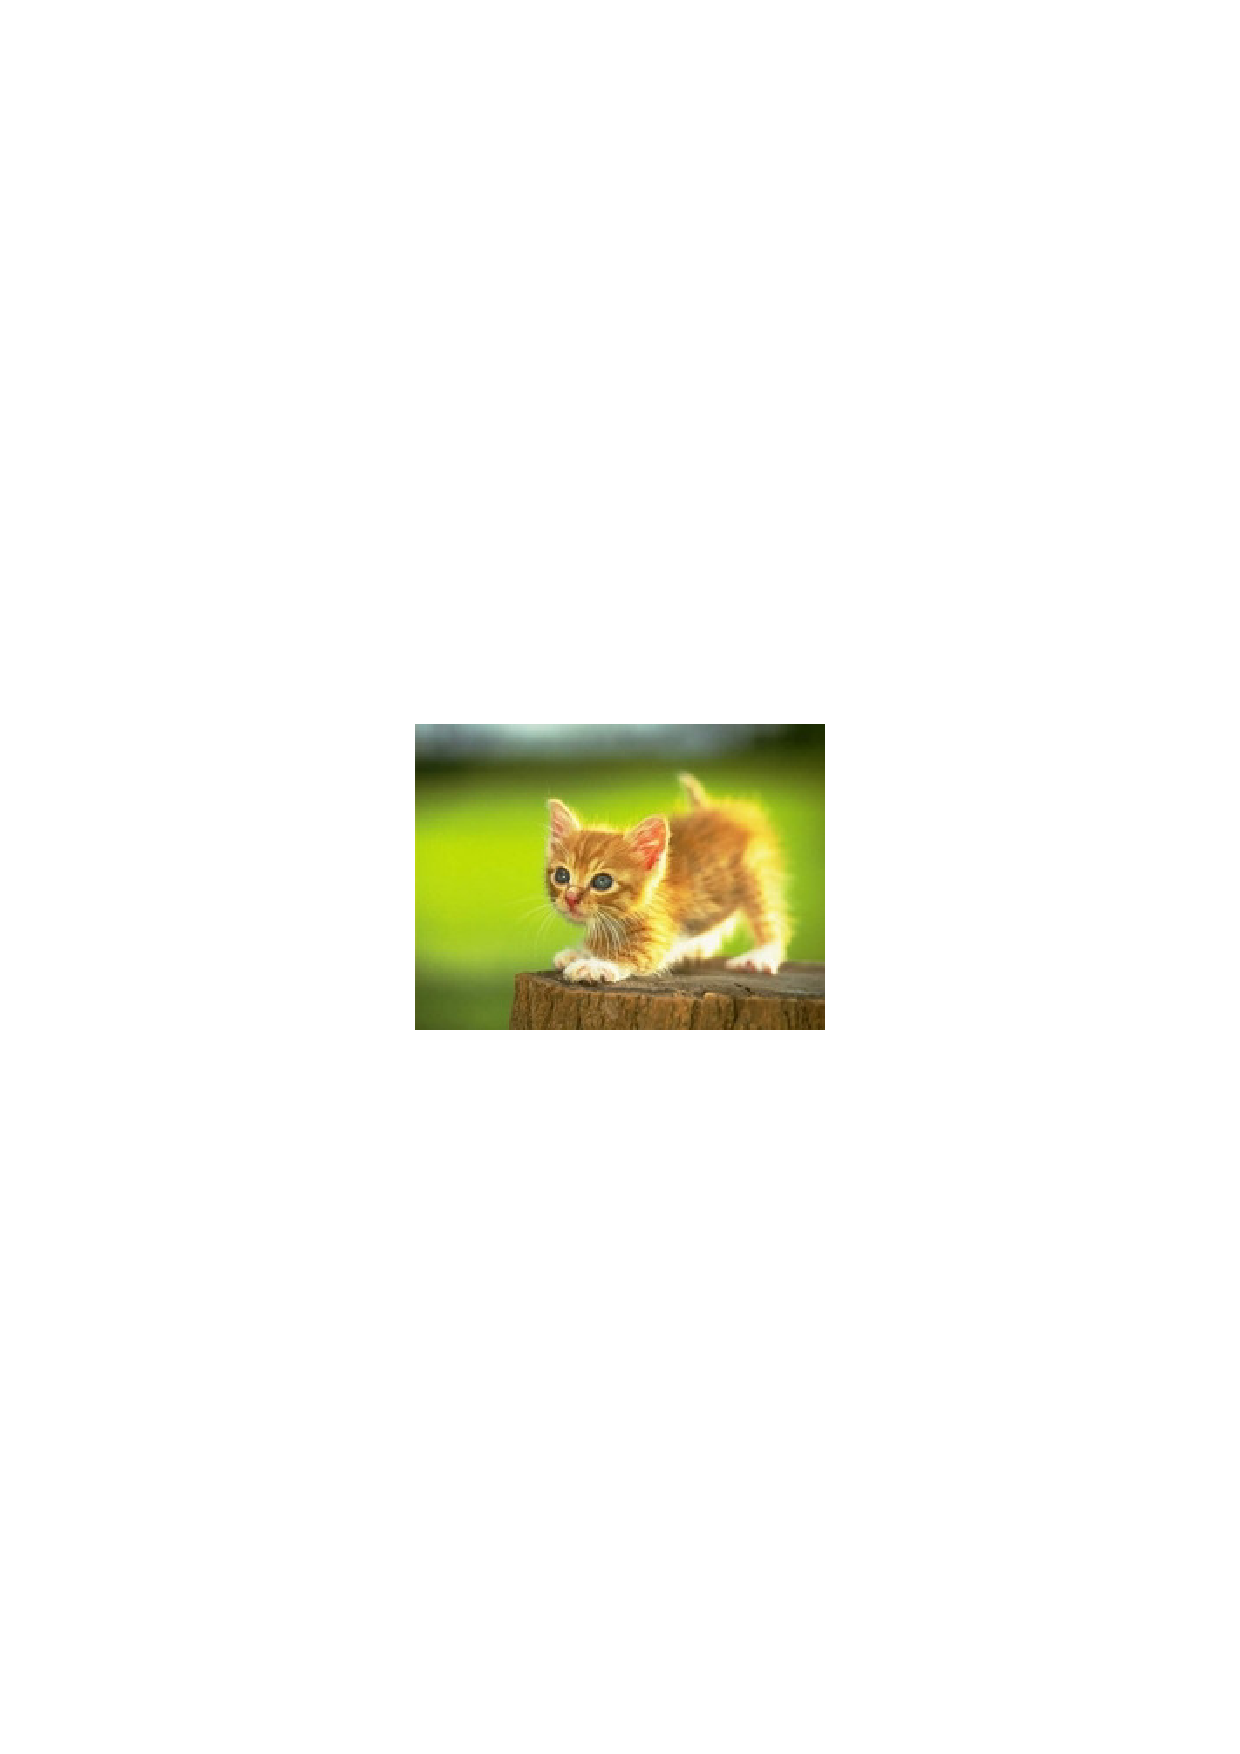
\includegraphics{cat}
\caption{一只猫的幸福}\label{fig:cat}
\end{figure}

四十年来家国,三千里地山河。 凤阁龙楼连霄汉,玉树琼枝作烟萝。
几曾识干戈。 一旦归为臣虏,沉腰潘鬓消磨。
最是仓皇辞庙日,教坊犹奏离别歌。 垂泪对宫娥。

是岁十月之望,步自雪堂,将归于临皋。二客从予过黄泥之坂。
霜露既降,木叶尽脱,人影在地,仰见明月,顾而乐之,行歌相答。
已而叹曰:“有客无酒,有酒无肴,月白风清,如此良夜何!”
客曰:“今者薄暮,举网得鱼,巨口细鳞,状如松江之鲈。顾安所得酒乎?”
归而谋诸妇。 妇曰:“我有斗酒,藏之久矣,以待子不时之需。”
于是携酒与鱼,复游于赤壁之下。江流有声,断岸千尺;山高月小,
水落石出。曾日月之几何,而江山不可复识矣。予乃摄衣而上,
履谗岩,披蒙茸,踞虎豹,登虬龙,攀栖鹘之危巢,俯冯夷之幽宫。
盖二客不能从焉。划然长啸,草木震动,山鸣谷应,风起水涌。予亦悄然而悲,
肃然而恐,凛乎其不可留也。反而登舟,放乎中流,听其所止而休焉。
时夜将半,四顾寂寥。适有孤鹤,横江东来。翅如车轮,玄裳缟衣,
戛然长鸣,掠予舟而西也。 须臾客去,予亦就睡。梦一道士,羽衣蹁跹,
过临皋之下,揖予而言曰:“赤壁之游乐乎?”问其姓名, 俯而不答。
“呜呼!噫嘻!我知之矣。畴昔之夜,飞鸣而过我者,非子也邪?”
道士顾笑,予亦惊寤。开户视之,不见其处。


\subsection{并排子图}

图~\ref{fig:cat1} 和~图~\ref{fig:cat2} 是位于浮动环境中的并列子图。
\begin{figure}[!htbp]%
\centering
\subfloat[一只猫的幸福]{\label{fig:cat1}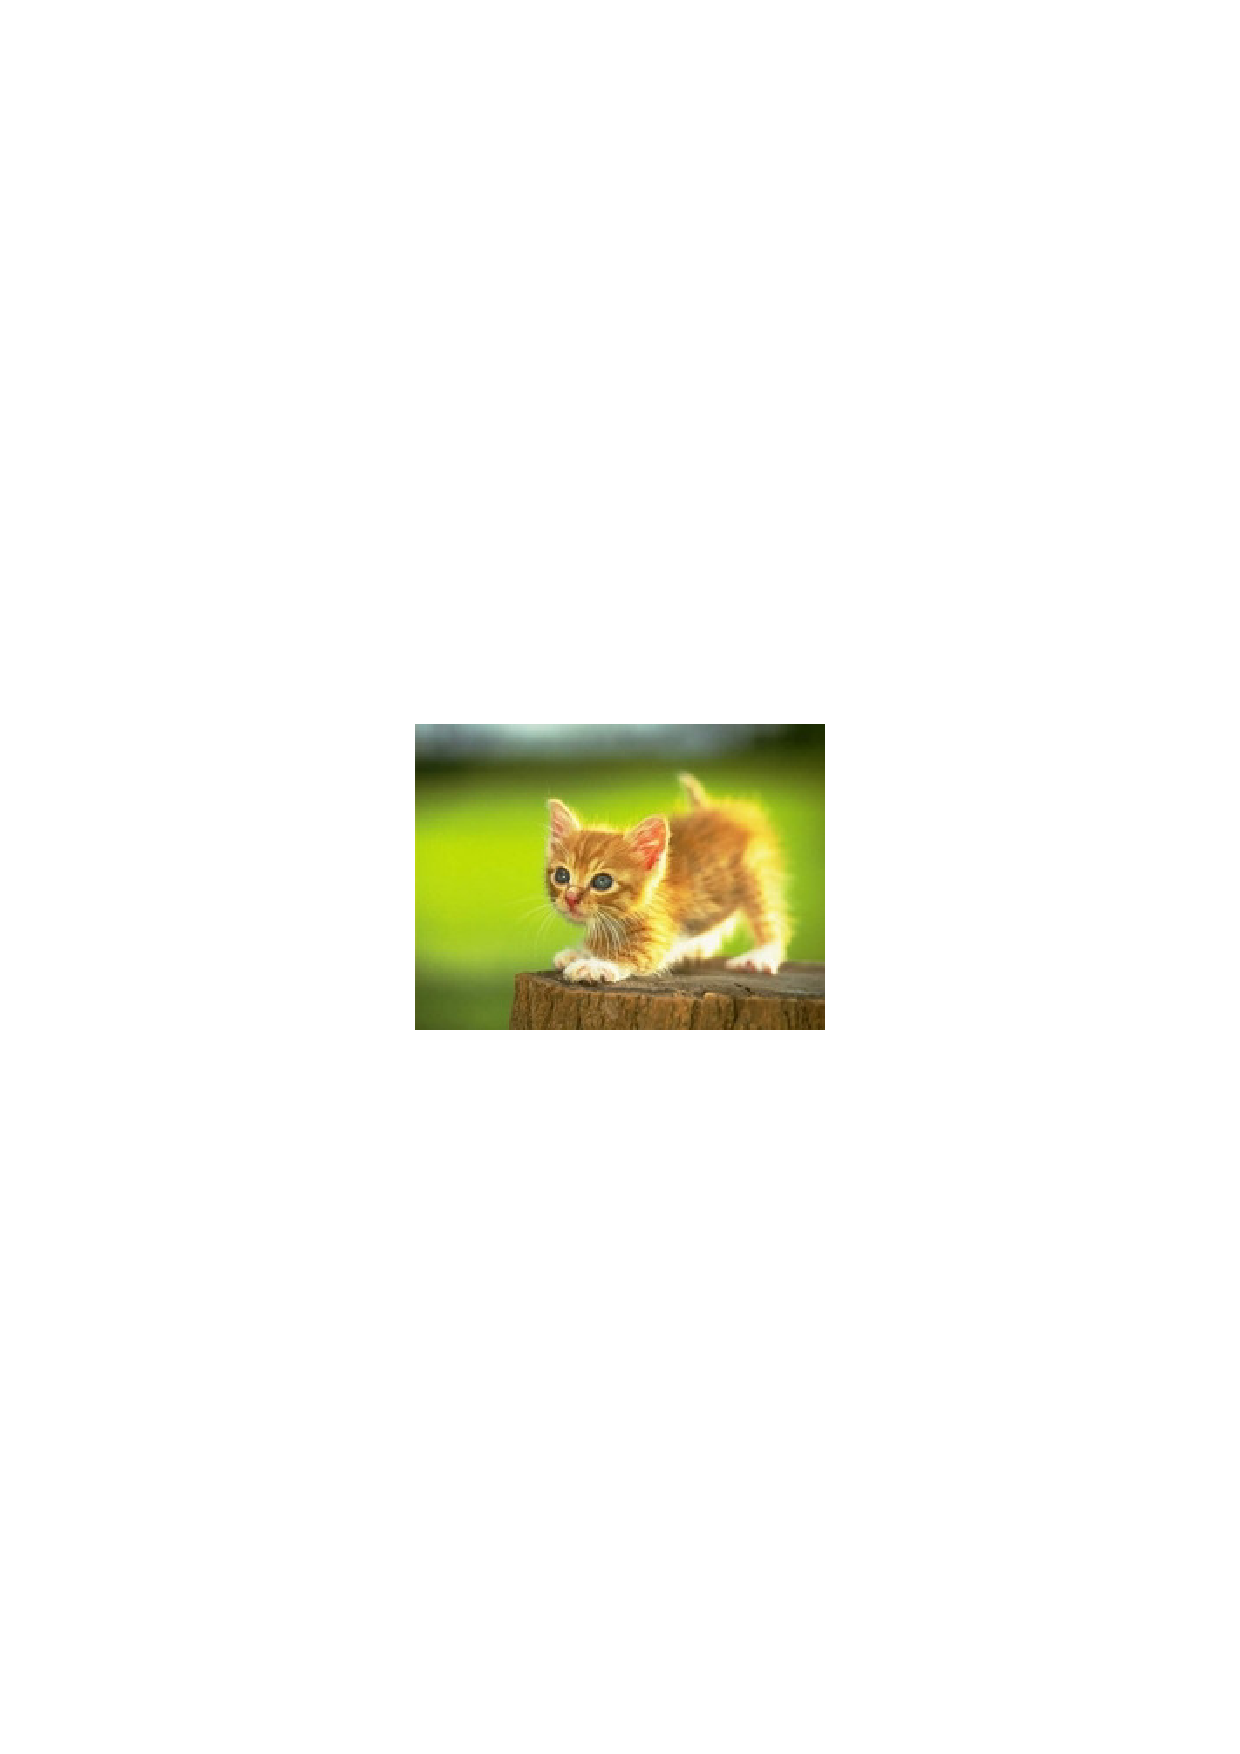
\includegraphics[scale=0.9]{cat}}%
\qquad
\subfloat[一只猫的幸福]{\label{fig:cat2}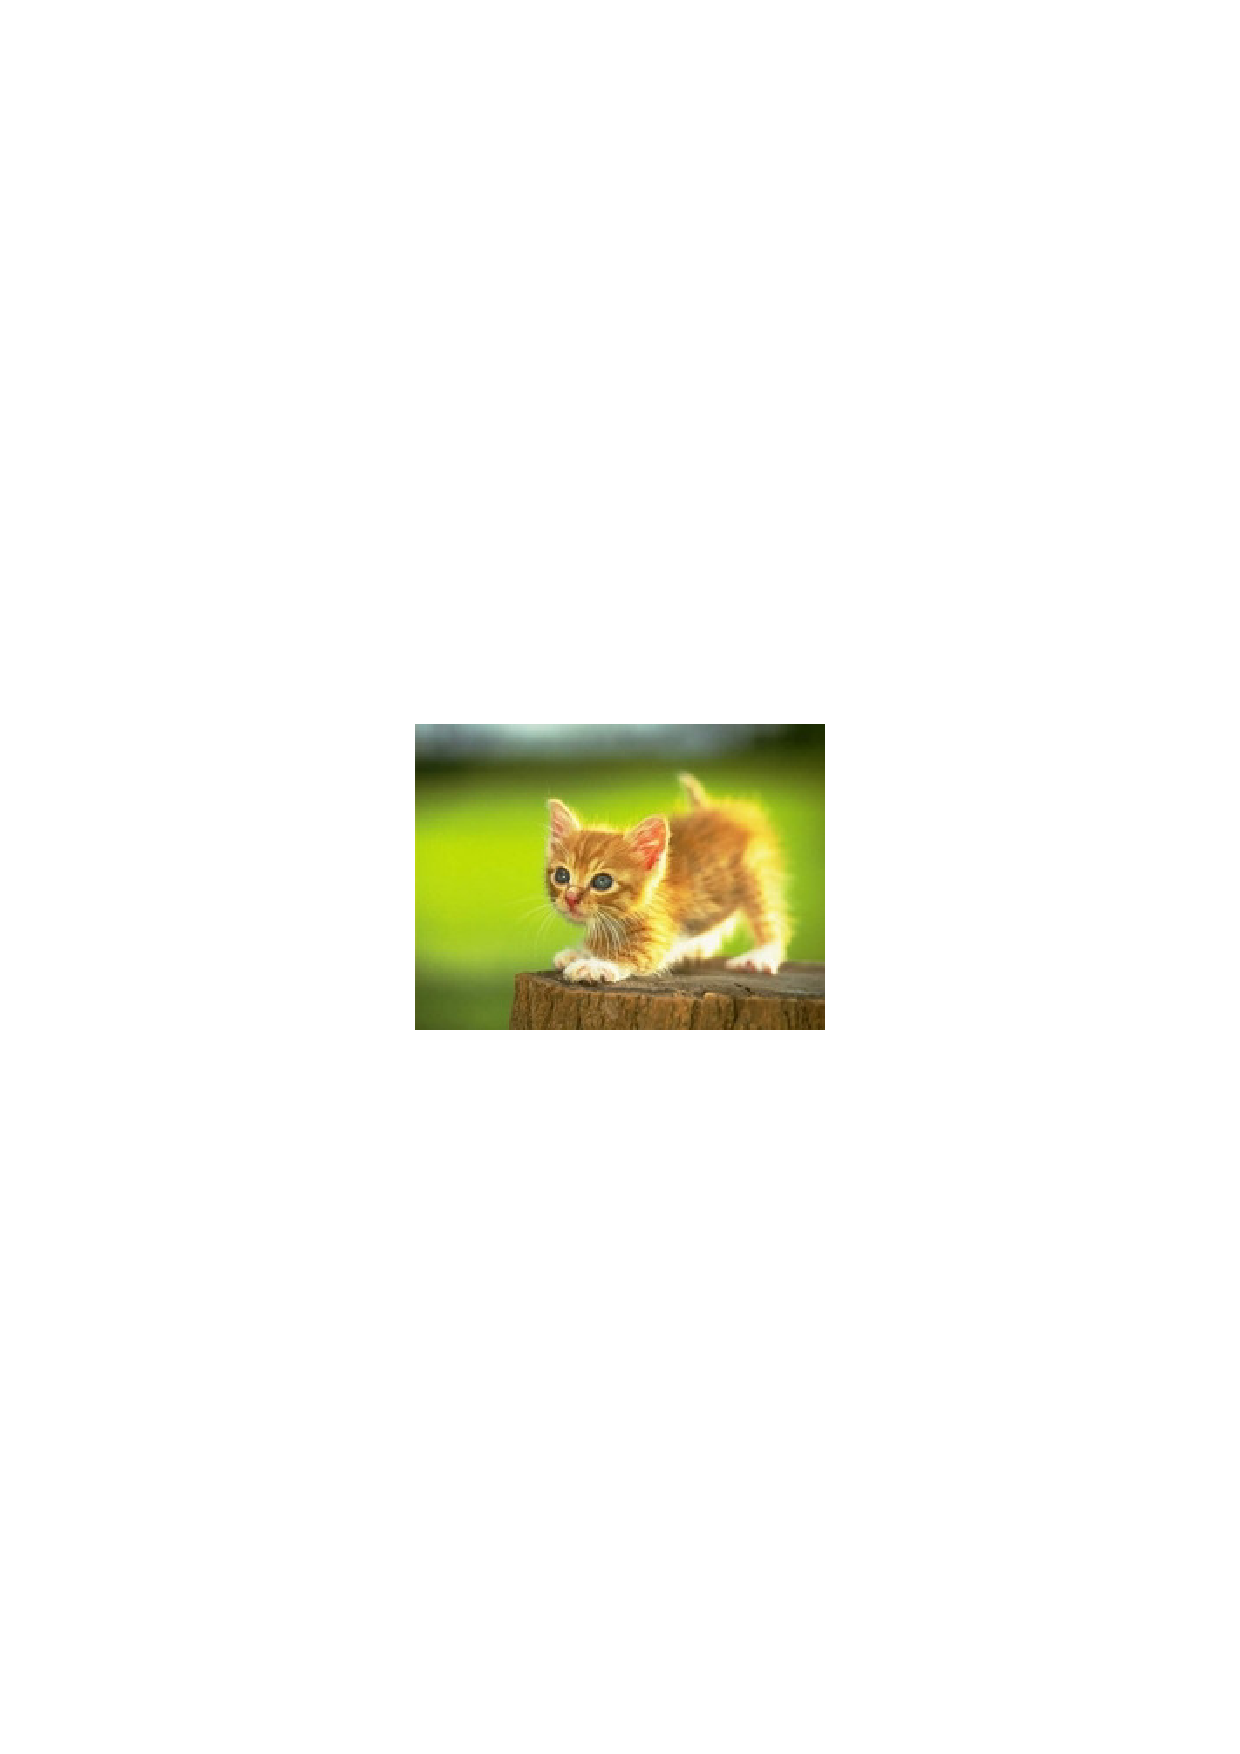
\includegraphics[scale=0.9]{cat}}%
\caption{A Tale of Two Kitties.}%
\end{figure}

月朦胧,鸟朦胧,点点萤火照夜空。 山朦胧,树朦胧,唧唧秋虫正呢哝。
花朦胧,叶朦胧,晚风轻轻叩帘栊。 灯朦胧,人朦胧,今宵但愿同入梦。
